% Options for packages loaded elsewhere
\PassOptionsToPackage{unicode}{hyperref}
\PassOptionsToPackage{hyphens}{url}
%
\documentclass[
]{article}
\usepackage{lmodern}
\usepackage{amssymb,amsmath}
\usepackage{ifxetex,ifluatex}
\ifnum 0\ifxetex 1\fi\ifluatex 1\fi=0 % if pdftex
  \usepackage[T1]{fontenc}
  \usepackage[utf8]{inputenc}
  \usepackage{textcomp} % provide euro and other symbols
\else % if luatex or xetex
  \usepackage{unicode-math}
  \defaultfontfeatures{Scale=MatchLowercase}
  \defaultfontfeatures[\rmfamily]{Ligatures=TeX,Scale=1}
\fi
% Use upquote if available, for straight quotes in verbatim environments
\IfFileExists{upquote.sty}{\usepackage{upquote}}{}
\IfFileExists{microtype.sty}{% use microtype if available
  \usepackage[]{microtype}
  \UseMicrotypeSet[protrusion]{basicmath} % disable protrusion for tt fonts
}{}
\makeatletter
\@ifundefined{KOMAClassName}{% if non-KOMA class
  \IfFileExists{parskip.sty}{%
    \usepackage{parskip}
  }{% else
    \setlength{\parindent}{0pt}
    \setlength{\parskip}{6pt plus 2pt minus 1pt}}
}{% if KOMA class
  \KOMAoptions{parskip=half}}
\makeatother
\usepackage{xcolor}
\IfFileExists{xurl.sty}{\usepackage{xurl}}{} % add URL line breaks if available
\IfFileExists{bookmark.sty}{\usepackage{bookmark}}{\usepackage{hyperref}}
\hypersetup{
  hidelinks,
  pdfcreator={LaTeX via pandoc}}
\urlstyle{same} % disable monospaced font for URLs
\usepackage[margin=1in]{geometry}
\usepackage{color}
\usepackage{fancyvrb}
\newcommand{\VerbBar}{|}
\newcommand{\VERB}{\Verb[commandchars=\\\{\}]}
\DefineVerbatimEnvironment{Highlighting}{Verbatim}{commandchars=\\\{\}}
% Add ',fontsize=\small' for more characters per line
\usepackage{framed}
\definecolor{shadecolor}{RGB}{248,248,248}
\newenvironment{Shaded}{\begin{snugshade}}{\end{snugshade}}
\newcommand{\AlertTok}[1]{\textcolor[rgb]{0.94,0.16,0.16}{#1}}
\newcommand{\AnnotationTok}[1]{\textcolor[rgb]{0.56,0.35,0.01}{\textbf{\textit{#1}}}}
\newcommand{\AttributeTok}[1]{\textcolor[rgb]{0.77,0.63,0.00}{#1}}
\newcommand{\BaseNTok}[1]{\textcolor[rgb]{0.00,0.00,0.81}{#1}}
\newcommand{\BuiltInTok}[1]{#1}
\newcommand{\CharTok}[1]{\textcolor[rgb]{0.31,0.60,0.02}{#1}}
\newcommand{\CommentTok}[1]{\textcolor[rgb]{0.56,0.35,0.01}{\textit{#1}}}
\newcommand{\CommentVarTok}[1]{\textcolor[rgb]{0.56,0.35,0.01}{\textbf{\textit{#1}}}}
\newcommand{\ConstantTok}[1]{\textcolor[rgb]{0.00,0.00,0.00}{#1}}
\newcommand{\ControlFlowTok}[1]{\textcolor[rgb]{0.13,0.29,0.53}{\textbf{#1}}}
\newcommand{\DataTypeTok}[1]{\textcolor[rgb]{0.13,0.29,0.53}{#1}}
\newcommand{\DecValTok}[1]{\textcolor[rgb]{0.00,0.00,0.81}{#1}}
\newcommand{\DocumentationTok}[1]{\textcolor[rgb]{0.56,0.35,0.01}{\textbf{\textit{#1}}}}
\newcommand{\ErrorTok}[1]{\textcolor[rgb]{0.64,0.00,0.00}{\textbf{#1}}}
\newcommand{\ExtensionTok}[1]{#1}
\newcommand{\FloatTok}[1]{\textcolor[rgb]{0.00,0.00,0.81}{#1}}
\newcommand{\FunctionTok}[1]{\textcolor[rgb]{0.00,0.00,0.00}{#1}}
\newcommand{\ImportTok}[1]{#1}
\newcommand{\InformationTok}[1]{\textcolor[rgb]{0.56,0.35,0.01}{\textbf{\textit{#1}}}}
\newcommand{\KeywordTok}[1]{\textcolor[rgb]{0.13,0.29,0.53}{\textbf{#1}}}
\newcommand{\NormalTok}[1]{#1}
\newcommand{\OperatorTok}[1]{\textcolor[rgb]{0.81,0.36,0.00}{\textbf{#1}}}
\newcommand{\OtherTok}[1]{\textcolor[rgb]{0.56,0.35,0.01}{#1}}
\newcommand{\PreprocessorTok}[1]{\textcolor[rgb]{0.56,0.35,0.01}{\textit{#1}}}
\newcommand{\RegionMarkerTok}[1]{#1}
\newcommand{\SpecialCharTok}[1]{\textcolor[rgb]{0.00,0.00,0.00}{#1}}
\newcommand{\SpecialStringTok}[1]{\textcolor[rgb]{0.31,0.60,0.02}{#1}}
\newcommand{\StringTok}[1]{\textcolor[rgb]{0.31,0.60,0.02}{#1}}
\newcommand{\VariableTok}[1]{\textcolor[rgb]{0.00,0.00,0.00}{#1}}
\newcommand{\VerbatimStringTok}[1]{\textcolor[rgb]{0.31,0.60,0.02}{#1}}
\newcommand{\WarningTok}[1]{\textcolor[rgb]{0.56,0.35,0.01}{\textbf{\textit{#1}}}}
\usepackage{longtable,booktabs}
% Correct order of tables after \paragraph or \subparagraph
\usepackage{etoolbox}
\makeatletter
\patchcmd\longtable{\par}{\if@noskipsec\mbox{}\fi\par}{}{}
\makeatother
% Allow footnotes in longtable head/foot
\IfFileExists{footnotehyper.sty}{\usepackage{footnotehyper}}{\usepackage{footnote}}
\makesavenoteenv{longtable}
\usepackage{graphicx,grffile}
\makeatletter
\def\maxwidth{\ifdim\Gin@nat@width>\linewidth\linewidth\else\Gin@nat@width\fi}
\def\maxheight{\ifdim\Gin@nat@height>\textheight\textheight\else\Gin@nat@height\fi}
\makeatother
% Scale images if necessary, so that they will not overflow the page
% margins by default, and it is still possible to overwrite the defaults
% using explicit options in \includegraphics[width, height, ...]{}
\setkeys{Gin}{width=\maxwidth,height=\maxheight,keepaspectratio}
% Set default figure placement to htbp
\makeatletter
\def\fps@figure{htbp}
\makeatother
\setlength{\emergencystretch}{3em} % prevent overfull lines
\providecommand{\tightlist}{%
  \setlength{\itemsep}{0pt}\setlength{\parskip}{0pt}}
\setcounter{secnumdepth}{-\maxdimen} % remove section numbering

\author{}
\date{\vspace{-2.5em}}

\begin{document}

\hypertarget{loesung-aufgabe-1.1}{%
\subsection{Loesung Aufgabe 1.1}\label{loesung-aufgabe-1.1}}

\begin{center}\rule{0.5\linewidth}{0.5pt}\end{center}

\begin{quote}
Download \href{13_Statistik1/RFiles/solution_stat1.R}{R-Skript}
\end{quote}

\begin{quote}
Download \href{13_Statistik1/RFiles/solution_stat1.pdf}{PDF}
\end{quote}

\begin{center}\rule{0.5\linewidth}{0.5pt}\end{center}

\textbf{kommentierte Musterlösungen}

\begin{Shaded}
\begin{Highlighting}[]
\CommentTok{# Als eine Möglichkeit, die Aufgabe 1.1 zu bearbeiten, nehmen wir hier den }
\CommentTok{# Datensatz  der Gästebefragung NOVANIMAL und gehen der folgenden Frage nach: }
\CommentTok{# Gibt es einen Zusammenhang zwischen Geschlecht und dem wahrgenommenen }
\CommentTok{# Milchkonsum (viel vs. wenig Milch/-produkte)}

\CommentTok{# die Variable wahrgenommener Milchkonsum muss noch in 2 Kategorien zusammengefasst werden: geringer vs. hoher Milchkonsum}


\CommentTok{# Variable  milk == wahrgenommener Milchkonsum }
\CommentTok{# alles kleiner als 4 (3 inklusive) == geringer wahrgenommener Milchkonsum, }
\CommentTok{#alles grösser als 3 (4 inklusive) == hoher wahrgenommener Milchkonsum}
\NormalTok{nova2 <-}\StringTok{ }\NormalTok{nova_survey }\OperatorTok\StringTok{ }
\StringTok{  }\KeywordTok{filter}\NormalTok{(gender }\OperatorTok{!=}\StringTok{ "x"}\NormalTok{) }\OperatorTok\StringTok{ }\CommentTok{# x aus der Variable Geschlecht entfernen }
\StringTok{  }\KeywordTok{mutate}\NormalTok{(}\DataTypeTok{milkcompt =} \KeywordTok{if_else}\NormalTok{(milk }\OperatorTok{>=}\StringTok{ }\DecValTok{3}\NormalTok{, }\StringTok{"wenig"}\NormalTok{, }\StringTok{"viel"}\NormalTok{)) }\OperatorTok\StringTok{ }
\StringTok{  }\KeywordTok{select}\NormalTok{(gender, milkcompt) }\OperatorTok\StringTok{ }
\StringTok{  }\KeywordTok{drop_na}\NormalTok{() }\CommentTok{# alle Missings können gestrichen werden}
 
    
\CommentTok{# mal anschauen}
\KeywordTok{table}\NormalTok{(nova2)}
\end{Highlighting}
\end{Shaded}

\begin{verbatim}
##       milkcompt
## gender viel wenig
##   Frau   23   469
##   Mann   25   623
\end{verbatim}

\begin{Shaded}
\begin{Highlighting}[]
\CommentTok{#Chi-squared Test}
\NormalTok{chi_sq <-}\StringTok{ }\KeywordTok{chisq.test}\NormalTok{(nova2}\OperatorTok{$}\NormalTok{gender, nova2}\OperatorTok{$}\NormalTok{milkcompt)}
\NormalTok{chi_sq}
\end{Highlighting}
\end{Shaded}

\begin{verbatim}
## 
##  Pearson's Chi-squared test with Yates' continuity correction
## 
## data:  nova2$gender and nova2$milkcompt
## X-squared = 0.28223, df = 1, p-value = 0.5952
\end{verbatim}

\begin{Shaded}
\begin{Highlighting}[]
\CommentTok{#Fisher's Test }
\KeywordTok{fisher.test}\NormalTok{(nova2}\OperatorTok{$}\NormalTok{gender, nova2}\OperatorTok{$}\NormalTok{milkcompt)}
\end{Highlighting}
\end{Shaded}

\begin{verbatim}
## 
##  Fisher's Exact Test for Count Data
## 
## data:  nova2$gender and nova2$milkcompt
## p-value = 0.5523
## alternative hypothesis: true odds ratio is not equal to 1
## 95 percent confidence interval:
##  0.6536644 2.2746745
## sample estimates:
## odds ratio 
##   1.221866
\end{verbatim}

\begin{center}\rule{0.5\linewidth}{0.5pt}\end{center}

\textbf{Ergebnisse}

Der \(\chi^2\)-Test sagt uns, dass das Geschlecht und der wahrgenommene
Milchkonsum nicht zusammenhängen. Es gibt keine signifikante
Unterscheide zwischen dem Geschlecht und dem wahrgenommenen Milchkonsum
(\(\chi^2\)(1) = 0.282, \emph{p} = 0.595. Es sieht so aus, dass Männer
leicht mehr angeben weniger Milch zu konsumieren (Tabelle 1). Die
Ergebnisse müssen jedoch mit Vorsicht interpretiert werden, denn der
\(\chi^2\)-Test gibt uns nur an, dass ein signifikanter Unterschied
zwischen Geschlecht und wahrgenommener Milchkonsum vorliegt. Um die
Unterschiede innerhalb der Gruppen (z.B. Geschlecht) festzustellen
bedarf es weiterer Analysen z. B. Odds Rations oder einer
mehrfaktorieller ANOVA mit anschliessenden Post-hoc Tests (siehe
Statistik 3).

\begin{verbatim}
## `summarise()` regrouping output by 'gender' (override with `.groups` argument)
\end{verbatim}

\begin{longtable}[]{@{}llrr@{}}
\caption{Wahrgenommener Milchkonsum nach Geschlecht}\tabularnewline
\toprule
Geschlecht & wahr. Milchkonsum & absolute Werte & wahr. Milchkonsum
(\%)\tabularnewline
\midrule
\endfirsthead
\toprule
Geschlecht & wahr. Milchkonsum & absolute Werte & wahr. Milchkonsum
(\%)\tabularnewline
\midrule
\endhead
Frau & viel & 23 & 4.7\tabularnewline
Frau & wenig & 469 & 95.3\tabularnewline
Mann & viel & 25 & 3.9\tabularnewline
Mann & wenig & 623 & 96.1\tabularnewline
\bottomrule
\end{longtable}

\hypertarget{musterloesung-aufgabe-1.2-t-test}{%
\subsubsection{Musterloesung Aufgabe 1.2:
t-Test}\label{musterloesung-aufgabe-1.2-t-test}}

\begin{quote}
Meine Empfehlung Kapitel 2 von
\href{https://mgimond.github.io/Stats-in-R/z_t_tests.html}{Manny Gimond}
\end{quote}

\textbf{Null- und Alternativhypothese} \(H_0\): Es gibt keine
Unterschiede in den Verkaufszahlen zwischen Basis- und
Interventionswochen.

\par

\(H_1\): Es gibt Unterschiede in den Verkaufszahlen zwischen Basis- und
Interventionswochen.

\begin{Shaded}
\begin{Highlighting}[]
\CommentTok{# Gemäss Aufgabenstellung müsset die Daten zuerst nach Kalenderwochen "week" }
\CommentTok{# und Bedingungen "condition" zusammengefasst werden}

\NormalTok{df <-}\StringTok{ }\NormalTok{nova }\OperatorTok
\StringTok{    }\KeywordTok{group_by}\NormalTok{(week, condit) }\OperatorTok\StringTok{  }
\StringTok{    }\KeywordTok{summarise}\NormalTok{(}\DataTypeTok{tot_sold =} \KeywordTok{n}\NormalTok{()) }
\end{Highlighting}
\end{Shaded}

\begin{verbatim}
## `summarise()` regrouping output by 'week' (override with `.groups` argument)
\end{verbatim}

\begin{Shaded}
\begin{Highlighting}[]
\CommentTok{# überprüft die Voraussetzungen für einen t-Test}
\KeywordTok{ggplot}\NormalTok{(df, }\KeywordTok{aes}\NormalTok{(}\DataTypeTok{x =}\NormalTok{ condit, }\DataTypeTok{y=}\NormalTok{ tot_sold)) }\OperatorTok{+}\StringTok{ }\CommentTok{# achtung 0 Punkt fehlt}
\StringTok{    }\KeywordTok{geom_boxplot}\NormalTok{(}\DataTypeTok{fill =} \StringTok{"white"}\NormalTok{, }\DataTypeTok{color =} \StringTok{"black"}\NormalTok{, }\DataTypeTok{size =} \DecValTok{1}\NormalTok{) }\OperatorTok{+}\StringTok{ }
\StringTok{    }\KeywordTok{labs}\NormalTok{(}\DataTypeTok{x=}\StringTok{"}\CharTok{\textbackslash{}n}\StringTok{Bedingungen"}\NormalTok{, }\DataTypeTok{y=}\StringTok{"Durchschnittlich verkaufte Gerichte pro Woche}\CharTok{\textbackslash{}n}\StringTok{"}\NormalTok{) }\OperatorTok{+}\StringTok{ }
\StringTok{    }\NormalTok{mytheme}
\end{Highlighting}
\end{Shaded}

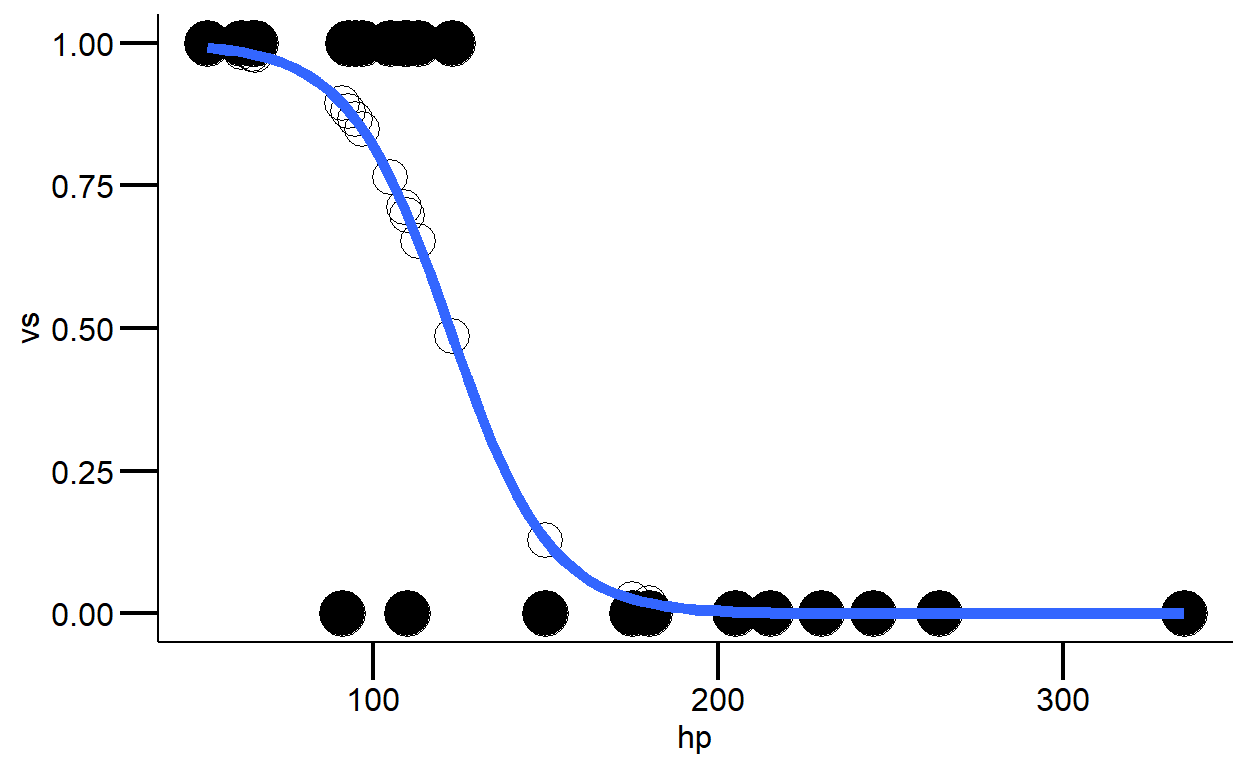
\includegraphics{solution_stat1_files/figure-latex/unnamed-chunk-4-1.pdf}

\begin{Shaded}
\begin{Highlighting}[]
\CommentTok{# Auf den ersten Blick scheint es keine starken Abweichungen zu einer }
\CommentTok{#Normalverteilung zu geben resp. es sind keine extremen schiefen Verteilungen}
\CommentTok{# ersichtlich (vgl. Skript Statistik 2)}
\end{Highlighting}
\end{Shaded}

\begin{Shaded}
\begin{Highlighting}[]
\CommentTok{# führt einen t-Tests durch; }
\CommentTok{# es wird angenommen, dass die Verkaufszahlen zwischen den Bedingungen }
\CommentTok{# unabhängig sind}

\NormalTok{t_test <-}\StringTok{ }\KeywordTok{t.test}\NormalTok{(tot_sold}\OperatorTok{~}\NormalTok{condit, }\DataTypeTok{data=}\NormalTok{df)}

\CommentTok{#alternative Formulierung}
\KeywordTok{t.test}\NormalTok{(df[df}\OperatorTok{$}\NormalTok{condit }\OperatorTok{==}\StringTok{ "Basis"}\NormalTok{, ]}\OperatorTok{$}\NormalTok{tot_sold, }
\NormalTok{                 df[df}\OperatorTok{$}\NormalTok{condit }\OperatorTok{==}\StringTok{ "Intervention"}\NormalTok{, ]}\OperatorTok{$}\NormalTok{tot_sold) }
\end{Highlighting}
\end{Shaded}

\begin{verbatim}
## 
##  Welch Two Sample t-test
## 
## data:  df[df$condit == "Basis", ]$tot_sold and df[df$condit == "Intervention", ]$tot_sold
## t = 0.27168, df = 9.9707, p-value = 0.7914
## alternative hypothesis: true difference in means is not equal to 0
## 95 percent confidence interval:
##  -115.2743  147.2743
## sample estimates:
## mean of x mean of y 
##      2203      2187
\end{verbatim}

\begin{center}\rule{0.5\linewidth}{0.5pt}\end{center}

\textbf{Methoden}

Ziel war es die aggregierten Verkaufszahlen zwischen den Interventions-
und Basiswochen zu vergleichen. Die Annahme war, dass die wöchentlichen
Verkaufszahlen unabhängig sind. Daher können die mittleren
Verkaufszahlen pro Woche zwischen den beiden Bedingungen mittels t-Test
geprüft werden. Obwohl die visuelle Inspektion keine schwerwiegenden
Verletzungen der Modelvoraussetzung zeigte, wurde einen Welch t-Test
gerechnet.

\begin{center}\rule{0.5\linewidth}{0.5pt}\end{center}

\textbf{Ergebnisse}

In den Basiswochen werden mehr Gerichte pro Woche verkauft als in den
Interventionsowochen (siehe Abbildung 1). Die wöchentlichen
Verkaufszahlen zwischen den Bedigungen (Basis oder Intervention)
unterscheiden sich gemäss Welch t-Test jedoch nicht signifikant
(\emph{t}(10) = 0.272 , \emph{p} = 0.791).

\begin{figure}
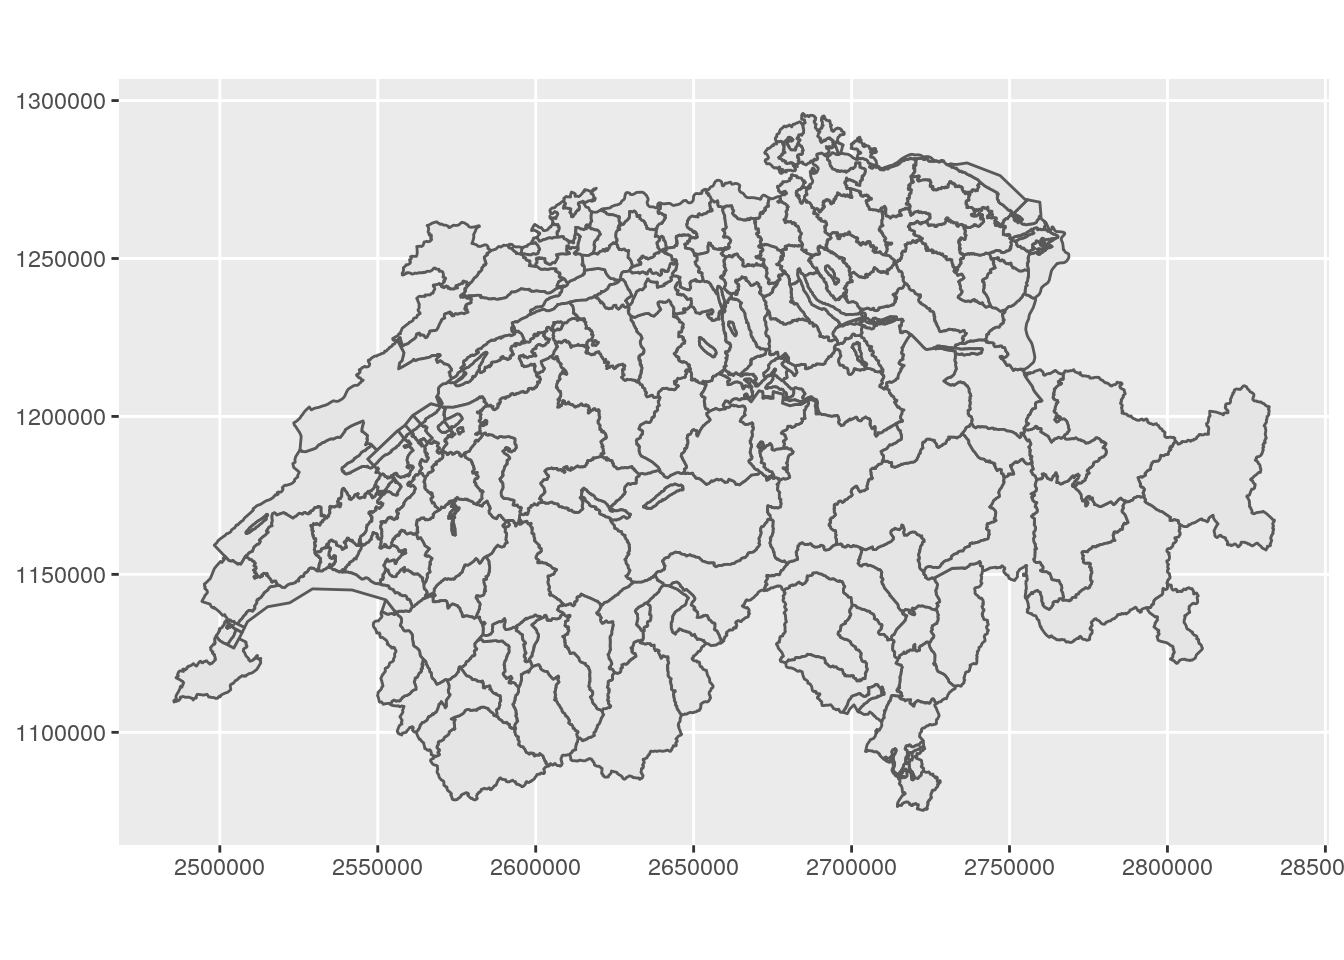
\includegraphics[width=0.8\linewidth]{solution_stat1_files/figure-latex/unnamed-chunk-6-1} \caption{Die wöchentlichen Verkaufszahlen für die Interventions- und Basiswochen unterscheiden sich nicht signifikant.}\label{fig:unnamed-chunk-6}
\end{figure}

\end{document}
